\documentclass[11pt,a4paper]{article}
\usepackage[T1]{fontenc}
\usepackage{lmodern}
\usepackage[margin=22mm]{geometry}
\usepackage{microtype}
\usepackage{booktabs}
\usepackage{graphicx}
\usepackage{titlesec}
\usepackage{fancyhdr}
\usepackage[hidelinks]{hyperref}
\hypersetup{pdftitle={Assignment 1 - Three Time Series Datasets}}
\setlength{\parindent}{0pt}
\setlength{\parskip}{5pt}
\renewcommand{\baselinestretch}{1.04}
\titleformat{\section}{\large\bfseries}{\thesection.}{0.6em}{}
\titlespacing*{\section}{0pt}{10pt}{7pt}
\pagestyle{fancy}
\fancyhf{}
\fancyfoot[L]{\footnotesize Data Forecasting - Assignment 1}
\fancyfoot[R]{\footnotesize\thepage}
\renewcommand{\headrulewidth}{0pt}
\renewcommand{\footrulewidth}{0pt}
\raggedbottom
\begin{document}
{\Large\bfseries Assignment 1: Time series datasets}\par
{\small Source snapshots retrieved 5 October 2026}\par
{\small Weekly, monthly and quarterly data; at least 100 observations each.
The two market datasets are multivariate; European macroeconomics adds a different domain.
All exported attributes have zero missing values. Calendar months and quarters are regular periods despite differing day counts.}\par

\section{NVIDIA stock}
{\small Weekly | Individual technology stock}\par
{\small\textbf{CSV:} \texttt{01\_nvda\_weekly.csv}\\
\textbf{Frequency:} Weekly\quad\textbf{Observations:} 312\quad\textbf{Attributes:} 3 (including date)\\
\textbf{Time span:} 2020-10-16 to 2026-10-02 (Friday labels)\\
Underlying trading dates: 2020-10-12 to 2026-10-02.}\par
\textbf{Sources.}\par
{\small\href{https://finance.yahoo.com/quote/NVDA/history/}{Yahoo Finance: NVDA historical data}\quad\url{https://finance.yahoo.com/quote/NVDA/history/}}\par
\textbf{Attributes and missing data.}\par
{\small\raggedright\texttt{date}: Friday labelling a Saturday-Friday week; YYYY-MM-DD. \mbox{Missing: 0.}\par}
{\small\raggedright\texttt{nvda\_adjusted\_close\_usd}: Last trading day's adjusted close in the week, USD per share. Yahoo adjusts this for splits and dividends. \mbox{Missing: 0.}\par}
{\small\raggedright\texttt{nvda\_volume\_shares}: Sum of the daily trading volumes reported by Yahoo within the week, in shares. \mbox{Missing: 0.}\par}
\textbf{Numeric summary.}\par
{\footnotesize\setlength{\tabcolsep}{3.5pt}\renewcommand{\arraystretch}{1.25}
\begin{tabular*}{\textwidth}{@{\extracolsep{\fill}}lrrrr@{}}
\toprule Attribute & Min & Max & Mean & Std. dev.\\ \midrule
\texttt{nvda\_adjusted\_close\_usd} & 11.19 & 233.95 & 82.12 & 70.38\\
\texttt{nvda\_volume\_shares} & 400,749,200.00 & 4,308,297,000.00 & 1,736,870,065.38 & 815,917,634.39\\
\bottomrule\end{tabular*}}\par
{\footnotesize Sample standard deviation ($n-1$); calculated from exported CSV values. Display rounded to two decimals.}\par
\textbf{Reduction and preparation.}\par
Daily observations were aggregated into Saturday-Friday weeks: last adjusted close and sum of volume. Only the most recent 312 complete weeks were retained. Open, high, low and unadjusted close were removed. A holiday Friday keeps the last actual quote within that week; the date is a period label. No prices were interpolated or forward-filled.\par
\textbf{Why this series is useful.}\par
An individual stock with strong trends and changing trading activity. Useful for studying price versus volume and the effect of differencing or returns on a trending series.\par
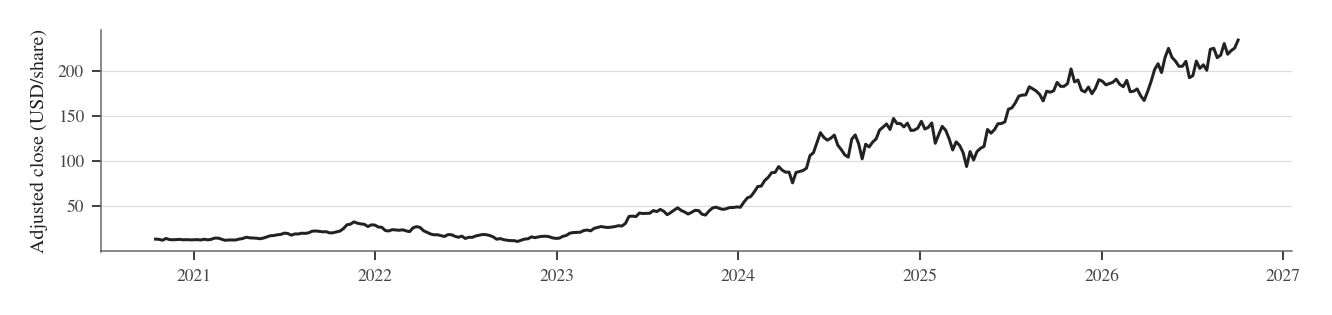
\includegraphics[width=\textwidth]{figures/series-1.png}
\newpage
\section{S\&P 500 and VIX}
{\small Monthly | Equity market level and expected volatility}\par
{\small\textbf{CSV:} \texttt{02\_sp500\_vix\_monthly.csv}\\
\textbf{Frequency:} Monthly\quad\textbf{Observations:} 108\quad\textbf{Attributes:} 4 (including date)\\
\textbf{Time span:} 2017-10-01 to 2026-09-01 (month-start labels)\\
Covered calendar months: 2017-10 through 2026-09, ending 2026-09-30.}\par
\textbf{Sources.}\par
{\small\href{https://finance.yahoo.com/quote/\%5EGSPC/history/}{Yahoo Finance: S\&P 500 historical data}\quad\url{https://finance.yahoo.com/quote/\%5EGSPC/history/}}\par
{\small\href{https://www.cboe.com/tradable\_products/vix/vix\_historical\_data}{Cboe: VIX historical data}\quad\url{https://www.cboe.com/tradable_products/vix/vix_historical_data}}\par
\textbf{Attributes and missing data.}\par
{\small\raggedright\texttt{date}: First day labelling the calendar month; YYYY-MM-DD. \mbox{Missing: 0.}\par}
{\small\raggedright\texttt{sp500\_mean\_close}: Arithmetic mean of the daily S\&P 500 closes, in index points; a price index excluding dividends. \mbox{Missing: 0.}\par}
{\small\raggedright\texttt{vix\_mean\_close}: Arithmetic mean of daily VIX closes, in volatility index points (annualized percentage units). \mbox{Missing: 0.}\par}
{\small\raggedright\texttt{vix\_max\_close}: Largest daily VIX close in the month, in the same units; this is not an intraday high. \mbox{Missing: 0.}\par}
\textbf{Numeric summary.}\par
{\footnotesize\setlength{\tabcolsep}{3.5pt}\renewcommand{\arraystretch}{1.25}
\begin{tabular*}{\textwidth}{@{\extracolsep{\fill}}lrrrr@{}}
\toprule Attribute & Min & Max & Mean & Std. dev.\\ \midrule
\texttt{sp500\_mean\_close} & 2,557.00 & 7,711.32 & 4,360.69 & 1,436.13\\
\texttt{vix\_mean\_close} & 10.13 & 57.74 & 19.35 & 6.62\\
\texttt{vix\_max\_close} & 11.30 & 82.69 & 24.51 & 10.14\\
\bottomrule\end{tabular*}}\par
{\footnotesize Sample standard deviation ($n-1$); calculated from exported CSV values. Display rounded to two decimals.}\par
\textbf{Reduction and preparation.}\par
Daily closes were grouped by calendar month: mean for each index and maximum daily close for VIX. The most recent 108 complete months were retained; incomplete October 2026 was excluded. Within this window, 33 extra VIX holiday observations were excluded to use the same S\&P 500 trading dates for both indexes. Other daily attributes were removed. No missing values were filled.\par
\textbf{Why this series is useful.}\par
A multivariate dataset contrasting broad equity-market trends with volatility spikes. The maximum VIX close retains information about stress that a monthly average can smooth out. No relationship between the variables is assumed.\par
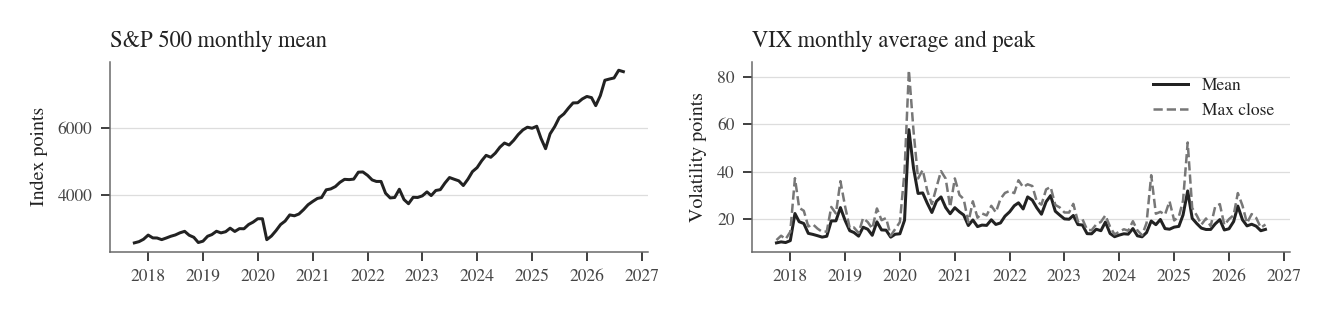
\includegraphics[width=\textwidth]{figures/series-2.png}
\newpage
\section{Euro-area real GDP index}
{\small Quarterly | European macroeconomics}\par
{\small\textbf{CSV:} \texttt{03\_euro\_area\_real\_gdp\_quarterly.csv}\\
\textbf{Frequency:} Quarterly\quad\textbf{Observations:} 120\quad\textbf{Attributes:} 2 (including date)\\
\textbf{Time span:} 1996-07-01 to 2026-04-01 (quarter-start labels)\\
Covered quarters: 1996Q3 through 2026Q2, ending 2026-06-30.}\par
\textbf{Sources.}\par
{\small\href{https://ec.europa.eu/eurostat/databrowser/view/namq\_10\_gdp/default/table?lang=en}{Eurostat: quarterly GDP (namq\_10\_gdp)}\quad\url{https://ec.europa.eu/eurostat/databrowser/view/namq_10_gdp/default/table?lang=en}}\par
\textbf{Attributes and missing data.}\par
{\small\raggedright\texttt{date}: First day labelling the quarter (January, April, July or October); YYYY-MM-DD. \mbox{Missing: 0.}\par}
{\small\raggedright\texttt{real\_gdp\_index}: Real GDP in chain-linked volumes, index 2020 = 100; seasonally and calendar adjusted. Covers the fixed 20-country euro-area group (EA20). Measures economic output excluding inflation. \mbox{Missing: 0.}\par}
\textbf{Numeric summary.}\par
{\footnotesize\setlength{\tabcolsep}{3.5pt}\renewcommand{\arraystretch}{1.25}
\begin{tabular*}{\textwidth}{@{\extracolsep{\fill}}lrrrr@{}}
\toprule Attribute & Min & Max & Mean & Std. dev.\\ \midrule
\texttt{real\_gdp\_index} & 74.33 & 114.67 & 95.81 & 10.51\\
\bottomrule\end{tabular*}}\par
{\footnotesize Sample standard deviation ($n-1$); calculated from exported CSV values. Display rounded to two decimals.}\par
\textbf{Reduction and preparation.}\par
Eurostat filters: frequency Q; geography EA20; GDP B1GQ; unit CLV\_I20; adjustment SCA. The selected source contains 126 quarters from 1995 Q1 through 2026 Q2; only the latest 120 were retained, removing the oldest six. Quarter codes were converted to quarter-start dates. Constant series metadata were omitted from the CSV. Original index values were preserved without aggregation or imputation.\par
\textbf{Why this series is useful.}\par
Adds a European economic domain and slower frequency. Useful for studying long-term growth, recessions and shocks such as the COVID-19 contraction and subsequent rebound. The source's seasonal and calendar adjustment helps focus on economic cycles.\par
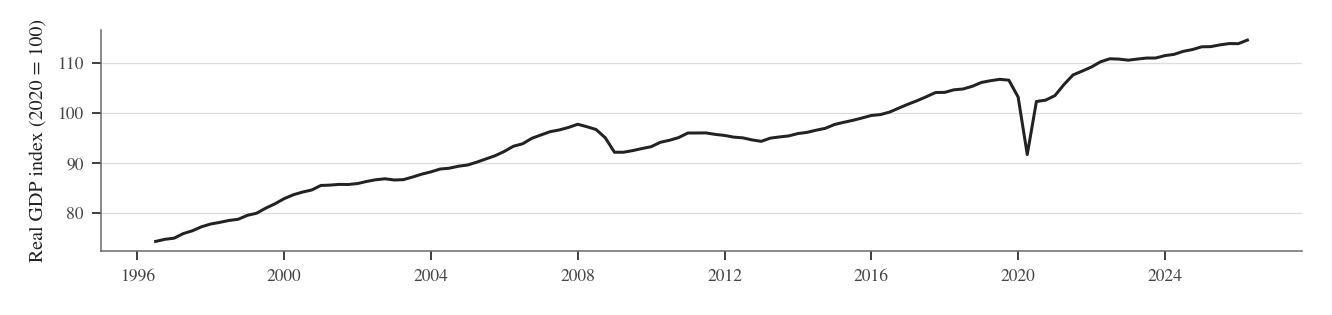
\includegraphics[width=\textwidth]{figures/series-3.png}
\end{document}
